
\chapter{The Regional Arctic System Model}
\label{chap:rasm}

I have used the Regional Arctic System Model as the main modeling tool in this dissertation.
RASM is a fully coupled regional earth system model applied over a large Pan-Arctic domain (Figure \ref{fig:rasm}b).
RASM was developed under the support of the United States Department of Energy.
The development of RASM has been motivated by the need to improve multi-decadal simulations of high-latitude climate and to advance our understanding of the coupled interactions between individual components within the Arctic climate system \citep{Roberts_2010}.
RASM combines the Weather Research and Forecasting (WRF) atmospheric model \citep{Skamarock_2008,Cassano_2016}, the Variable Infiltration Capacity (VIC) hydrology model \citep{Hamman_2016a,Liang_1994,Liang_1996}, the RVIC streamflow routing model \citep{Hamman_2016b,Lohmann_1996}, the Parallel Ocean Program (POP) model \citep{Smith_2010}, and the Los Alamos Sea Ice (CICE) model \citep{Roberts_2015a,Hunke2013,Hunke2015} using the Community Earth System Model (CESM) coupling infrastructure \citep{Craig_2012}.
Additional details describing the specific application of each of the RASM component models can be found in the following chapters as well as in the RASM-specific cited literature above.

\begin{figure}
  \centering
  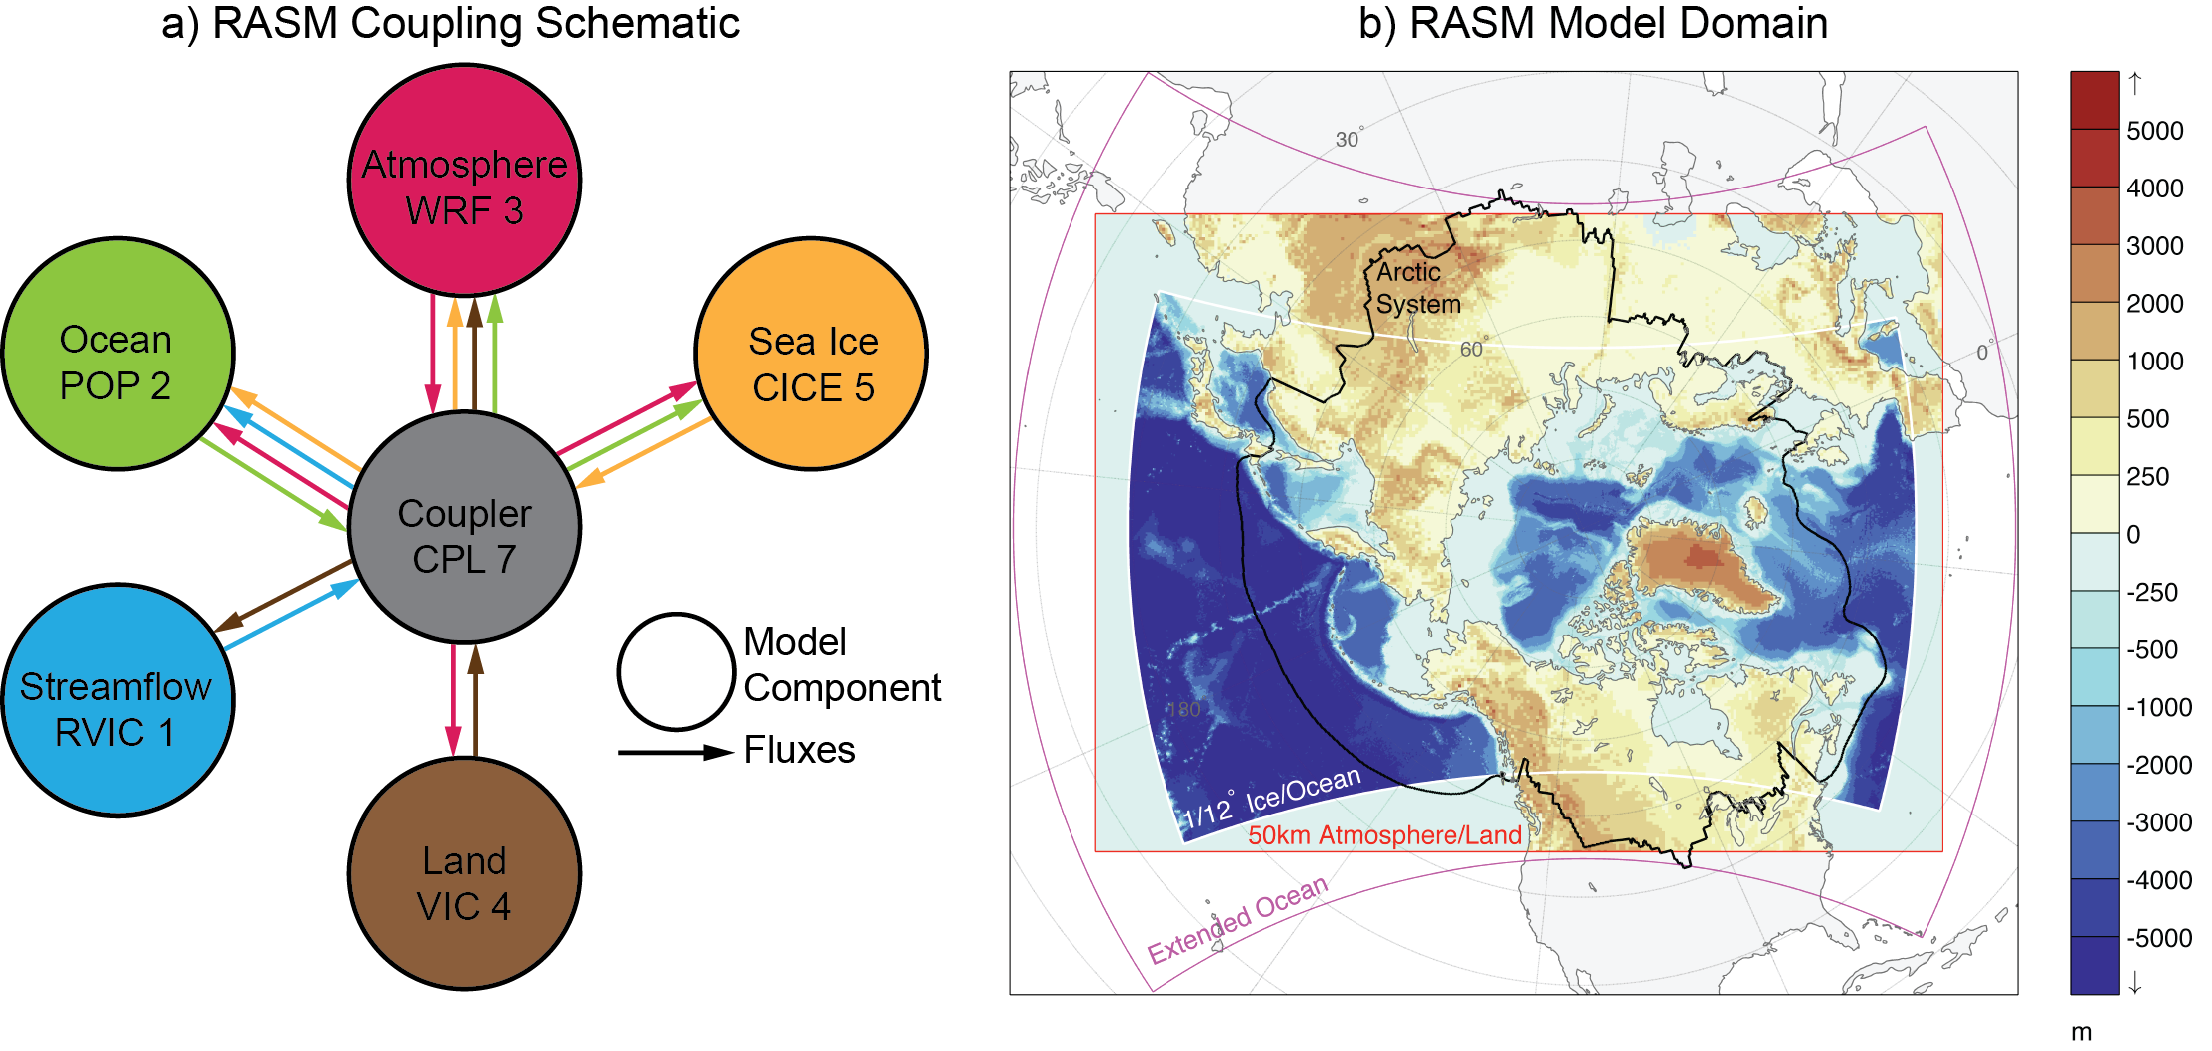
\includegraphics[width=12cm,keepaspectratio]{rasm_schematic_domain}
  \caption{a) Schematic of model configuration in RASM.
  The CPL7 flux coupler passes and receives all fluxes, shown with color coded arrows based on their source model, transferred across model boundaries.
  The component land, atmosphere, ocean, and sea ice models each calculate internal physics apart from the coupler.
  b) RASM model domain.
  There are three main grid domains in RASM, 1/12$^{\circ}$ rotated pole ice/ocean, a 50-km near equal area polar stereographic atmosphere/land/streamflow, and 1/12$^{\circ}$Extended Ocean.
  The color bar represents elevation above or below sea level.
  The black outline designates the greater Arctic Basin.}
  \label{fig:rasm}
\end{figure}

The RASM domain includes the entire Arctic drainage basin and encompasses the historical extent of seasonal sea ice cover.
For the work presented in this dissertation, RASM is applied exclusively over a 50-km near equal-area stereographic grid (Figure \ref{fig:rasm}b).
The individual model components (Figure \ref{fig:rasm}a) in RASM are tightly-coupled in RASM, exchanging flux variables though the flux coupler every 20 minutes.
This coupling configuration is described by \citet{Roberts_2015a}, where the sub-daily coupling frequency is shown to be important in reproducing observed inertial frequencies in the atmosphere-ice-ocean coupling cycle.

The development and use of a regional climate model, such as RASM, has advantages and disadvantages when compared to global climate model (GCMs).
Most notably, from a computational perspective, regional models are applied over a smaller region than global models, they may be run at higher spatial and temporal resolutions.
Higher resolution is generally thought to improve model representation of certain processes, such as orographic precipitation, coastal processes, and mesoscale processes \citep{Feser_2011}.
Another way to think of how high-resolution regional models are useful is as a testbed for future global model parameterizations.
As global models trend to higher resolutions, parameterizations related to model dynamics (e.g. ocean eddies, clouds, convective precipitation) will need to be re-evaluated; regional models offer a way to test out new combinations of parameterizations \citep[e.g. ][]{Roberts_2015a,Cassano_2016}.
Regional models must be forced at their lateral boundaries with output from a global model (either reanalysis or a GCM).
In some cases, this can be viewed as a disadvantage of using a regional model since global climate feedbacks are not accounted for.
Conversely, forcing regional models at their boundaries limit the degrees of freedom in the climate system, which can be viewed as an advantage when interpreting the response of new model parameterizations.

RASM version 1.0 was completed in 2015 and since then it has been used in a range of applications.
\citet{Roberts_2015a} used RASM to develop refined ice-ocean-atmosphere coupling scheme at sub-hourly timesteps.
They went on to show how this improvement leads to better simulation of semi-diurnal sea ice drift in RASM and in a GCM.
\citet{Cassano_2016} used RASM to evaluate a range of sea ice, ocean, and atmospheric parameterizations in terms of their impact on radiation biases.
This dissertation (chapters \ref{chap:land_surface}, \ref{chap:streamflow}, and \ref{chap:winter_prec}) represent the existing body of work related to the development and evaluation of the land surface within RASM.
